\documentclass{article}
\title{Sections and Chapters}
\author{Overleaf}
\date{\today}
\usepackage{hyperref}
\usepackage{graphicx}
\usepackage{float}
\usepackage[scriptsize]{caption}


\hypersetup{
    colorlinks,
    citecolor=black,
    filecolor=black,
    linkcolor=black,
    urlcolor=blue
} 
    
\urlstyle{same}

\begin{document}
\phantomsection
\addcontentsline{toc}{section}{Front Page}
\section*{Front Page}
\pagebreak


{\Large \bf\tableofcontents}
\phantomsection
\addcontentsline{toc}{section}{Table Of Contents}

\pagebreak
\phantomsection
\addcontentsline{toc}{section}{Introduction}
\section*{\LARGE Introduction}
\large The project called the Supermarket Management System works with supermarket automation and covers both the managing and selling of goods. 
\newline
The purpose of this project is to improve the existing system by making it more accurate, dependable, quick, and simple. There are various reasons for launching the project, including the numerous inefficiencies that salespeople deal with when selling products using the manual technique as humans are bound to make mistakes sooner or later. Thus, this is where the software will come handy.

\\
\phantomsection
\addcontentsline{toc}{section}{About}
\section*{\LARGE About}
\large A Supermarket Management System is a software application enabling management of products and selling them easily without the need to do calculations manually.
\newline
Generally, the software will provide a friendly user interface to add or remove or sell products and upon selling will automatically update the existing inventory.
\newline
\large{\href{https://github.com/mahirshahriar1/CSE_215_Project}{\\Click here to access Github} }
\newline
\large{\href{https://trello.com/b/mirX8zh2/cse215project}{\\Click here to access Trello} }
\\
\addcontentsline{toc}{section}{Purpose}
\section*{\LARGE Purpose and benefits of Supermarket Stock Management Project}
\large The purpose behind the creation of this software was to make things easier and error free. Owner of supermarkets often face difficulties on keeping a track of the inventory. The staffs also waste a lot of time adding the total of the selling products and making an invoice. Thus, arose the need of a management software.


\phantomsection
\addcontentsline{toc}{section}{Some benefits and Features}
\section*{\LARGE Some benefits and Features of Supermarket Stock Management}
\large 
\begin{itemize}
    \item \large Easy to add/edit product.
    \item \large No chance of duplicate IDs of product. (The software will not allow it)
    \item \large Can easily check which product is not currently at stock. This allows the employee to make a list of products that needs to be restocked. 
    \item \large Sorting features available by which the user can easily check the products according to his/her needs. 
    \item \large Saves time as everything is automated. 
    \item \large While selling products to a customer, the staff just needs to select the product and write the quantity. The invoice will be automatically generated upon pressing a sell button. The invoice is also printable, and can be saved in a database for future purpose.
    \item \large Once some products are sold, no one needs to update the inventory. The inventory is automatically updated.
    \item \large Less chances of any kind of errors as the software handles most types of cases where an error might have been made. (Negative amount/more quantity sold than available/ wrong calculation of tax or summation of products)
    \item \large User Friendly Graphical Interface which is easy to use.
    
\end{itemize}

\pagebreak


\phantomsection
\addcontentsline{toc}{section}{User Story}
\section*{\LARGE User Story}
\large 
\begin{itemize}
    \item \large \underline{\textbf{Use Case 1:}}\\\\
Mr. Xyz, the Admin of a shop need to assign a new employee or a staff. He logs in to his account where he finds a button “Add Employee” . Then he can add an employee. The ID needs to be unique, if not, then the software will show an error message.\\
    \item \large \underline{\textbf{Use Case 2:}}\\\\
    Mr. Xyz, the Admin of a shop needs to edit information of an employee or a staff. He chooses the option to edit the employee/staff and there he will find a list with all information which he can change. Only the admin can change the password of employee/staff account.\\
    \item \large \underline{\textbf{Use Case 3:}}\\\\
    The admin can see the list of products and can tell the employee to make necessary changes on the inventory.\\
    \item \large \underline{\textbf{Use Case 4:}}\\\\
    Employee A checks the message from the admin then he goes to the edit products option where he finds a list of all the products. Then he selects a product to which he wants to make some changes and presses the save button.\\
    \item \large \underline{\textbf{Use Case 5:}}\\\\
    Employee A receives some new products from the supplier and wants to add them to the stock list. He presses the Add Product option in the software and there he can add the product by filling the necessary options.\\
    \item \large \underline{\textbf{Use Case 6:}}\\\\
    A customer goes to Staff X at the counter in the shop with products they want to purchase. Staff A identifies the product by looking at the ID sticker of the product and selects those items to sell. Then the software will generate an invoice once the staff clicks on sell button.\\

\end{itemize}
\phantomsection
\addcontentsline{toc}{section}{Target Customers}
\section*{\LARGE Target Customers}
\large 
\begin{itemize}
    \item \large Any Supermarket Owners can use this software without any further changes. 
    \item \large Other Product Selling Companies can also adopt this software in their management with little changes made in the interface.
\end{itemize}

\phantomsection
\addcontentsline{toc}{section}{Software Features and Descriptions}
\section*{\LARGE Software Features and Descriptions}
The software will open with a Login Page where the user needs to select Admin/Employee/Staff. Then enter their respective ID and Password \\

\textbf {\Large Admin's screen will have:}
\begin{itemize}
    \item \large Add Employee.
    \item \large Add Staff.
    \item \large Edit Employee.
    \item \large Edit Staff.
    \item \large See Products.
    \item \large Send Message to Employee.  \\
\end{itemize} 
\pagebreak

\textbf {\Large Employee's screen will have:}
\begin{itemize}
    \item \large Check Messages.
    \item \large Add Products.
    \item \large Edit Products.
    \item\large  See Products.\\
\end{itemize} 

\textbf {\Large Staff's screen will have:}
\begin{itemize}
    \item\large  See Products.
    \item \large Sell Products.\\
\end{itemize} 
\textbf {\Large Some Features:}
\begin{itemize}
    \item\large  Products can be searched using ID.
    \item \large Invoice is Generated after selling.
    \item \large No duplicate IDs of anything\\
\end{itemize} 

\phantomsection
\addcontentsline{toc}{section}{Limitations of the project}
\section*{\LARGE Limitations of the project}
\large 
\begin{itemize}
    \item \large The data is stored locally. So, the data is at risk and vulnerable. 
    \item \large Does not have a Bar/QR code feature which would make product identification much faster.
\end{itemize}

\phantomsection
\addcontentsline{toc}{section}{Tools And Technologies}
\section*{\LARGE Tools And Technologies}
\large 
\begin{itemize}
    \item \large Java.
    \item \large Java Swing.
    \item \large Latex.
\end{itemize}
\pagebreak

\phantomsection
\addcontentsline{toc}{section}{Updates after Designing}
\section*{\LARGE Updates made in the project after Project Designing}
Some classes were added to sort the products.\\
And instead of the invoice class, a Cart class were created where the staff added the products that were being sold. Upon selling It generated an invoice using a jFrame. 

  \begin{figure}[htp]
 \centering
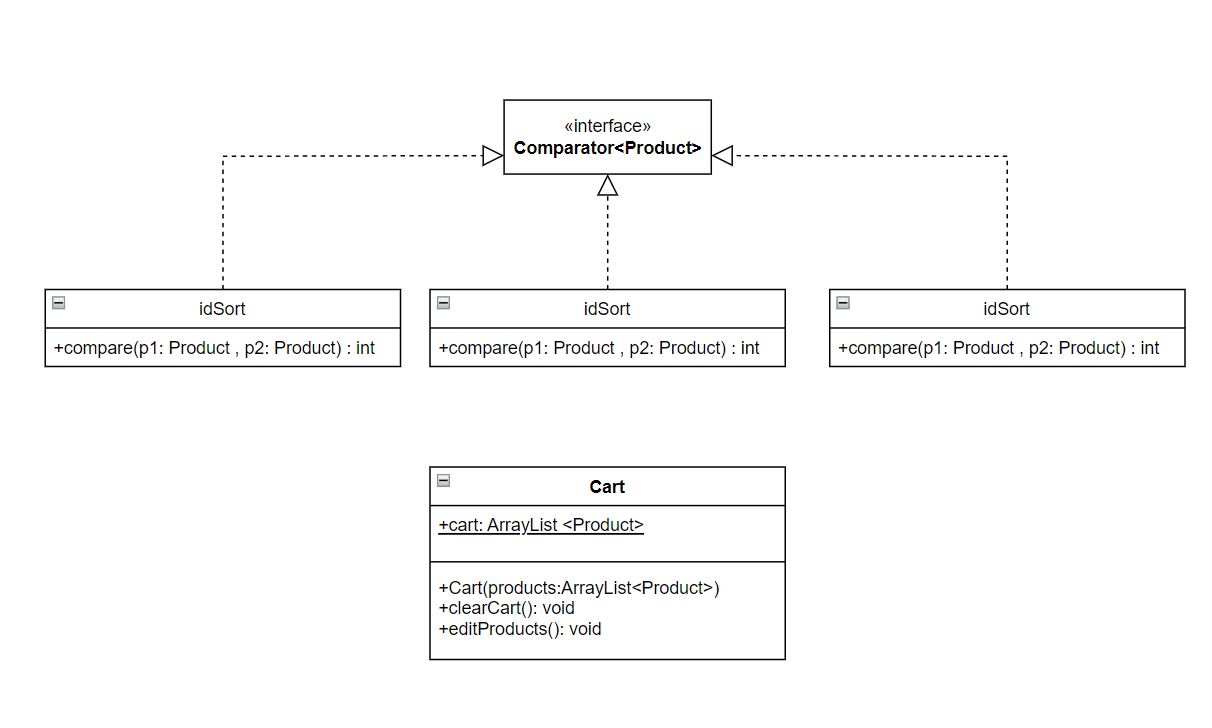
\includegraphics[scale=.45]{Capture.PNG}  
\end{figure}

A few other adjustments have been method in other Classes to while developing.

\pagebreak

\phantomsection
\addcontentsline{toc}{section}{Screenshots of Project}
\section*{\LARGE Screenshots of Project}

\pagebreak
ss\\ \newpage
ss
\pagebreak
\phantomsection
\addcontentsline{toc}{section}{Project Timeline}
\section*{\LARGE Project Timeline}
\large 
\begin{itemize}
    \item \large Day 1-2: Project Proposal.
    \item \large Day 2-4: Project Designing.
    \item \large Day 5-10: Both Developers Worked on the the project's code.
    \item \large Day 11-12: Checked for Errors in the project and fixed them.
    \item \large Day 13: Designed the GUI to make it User Friendly.
    \item \large Day 14: Project Report.
\end{itemize}

\phantomsection
\addcontentsline{toc}{section}{Possible Future Updates}
\section*{\LARGE Possible Future Updates}
This might not be the best solution for the given problem, but it will drastically change the experience of management and save a lot of time either way. A few further updates can be made upon user reviews and feed-backs and if the data is linked with an online platform, the data will be secure and safer.
\\
\\

\phantomsection
\addcontentsline{toc}{section}{Conclusion}
\section*{\LARGE Conclusion}
The goal of this project was to make the management system more accurate, dependable, quick, and simple. It was launched for a variety of reasons, including the numerous inefficiencies that salespeople face when selling products manually, as humans are not perfect. As a result, the software will be useful in this situation to avoid mistakes and save a lot of time.





\end{document}
